% !TEX TS-program = pdflatex
% !TEX encoding = UTF-8 Unicode

\documentclass{beamer}
\mode<presentation>
{
  \usetheme{Warsaw}

  \setbeamercovered{transparent}
  % or whatever (possibly just delete it)
}

\usepackage[english]{babel}

\usepackage[utf8]{inputenc}
% or whatever

%\usepackage{palatino}
%\usepackage[T1]{fontenc}
% Or whatever. Note that the encoding and the font should match. If T1
% does not look nice, try deleting the line with the fontenc.

%%%%%%%%%%%%%%%%%%%%%%%%%%%%%%%%%%%
\usepackage{graphicx}
\usepackage{wrapfig}
%%%%%%%%%%%%%%%%%%%%%%%%%%%%%%%%



\title{Entropy, Fractals, \& Extraterrestrial Life}

%\subtitle
%{Presentation Subtitle} % (optional)

\author{D. Baron}
% - Use the \inst{?} command only if the authors have different
%   affiliation.

\institute[Western Washington University] % (optional, but mostly needed)
{ Department of Mathematics\\
  Western Washington University}
% - Use the \inst command only if there are several affiliations.
% - Keep it simple, no one is interested in your street address.

\date{May 16, 2016}

\subject{Mathematical Astrobiology}
% This is only inserted into the PDF information catalog. Can be left
% out. 



% Delete this, if you do not want the table of contents to pop up at
% the beginning of each subsection:
\AtBeginSubsection[]
{
  \begin{frame}<beamer>{Outline}
    \tableofcontents[currentsection,currentsubsection]
  \end{frame}
}


% If you wish to uncover everything in a step-wise fashion, uncomment
% the following command: 

%\beamerdefaultoverlayspecification{<+->}


%%%%%%%%%%%%%%%%%%%
\newcommand{\newc}{\newcommand}
\newc{\Frame}[2]{\begin{frame}{#1}
#2
\end{frame}}
\newc{\lrp}[1]{\left(#1\right)}
\newc{\lrc}[1]{\left\{#1\right\}}
\newc{\al}[1]{\begin{align*}#1\end{align*}}
\newc{\defin}{\textbf{Definition. }}
\newc{\R}{\mathbb{R}}
\newc{\N}{\mathbb{N}}
\newc{\E}{\mathbb{E}}
\newc{\RR}{$\R$}
\newc{\lrb}[1]{\left[#1\right]}
\newc{\Db}{D_{\mathrm{box}}}
\newc{\db}{d_{\mathrm{box}}}
\DeclareMathOperator{\fe}{fe}
\DeclareMathOperator{\FE}{FE}
\DeclareMathOperator{\FS}{FS}
\newc{\bits}{\ \text{bits}}
\newc{\Ne}{N(\epsilon)}
\newc{\eps}{\epsilon}
\newc{\ent}[1]{H\!\lrp{#1}}
\newc{\entsum}[2]{-\sum_{#1}p(#2)\log p(#2)}
%%%%%%%%%%%%%

\begin{document}

\begin{frame}
  \titlepage
\end{frame}

%\begin{frame}{Outline}
%  \tableofcontents
%  % You might wish to add the option [pausesections]
%\end{frame}


% Since this a solution template for a generic talk, very little can
% be said about how it should be structured. However, the talk length
% of between 15min and 45min and the theme suggest that you stick to
% the following rules:  

% - Exactly two or three sections (other than the summary).
% - At *most* three subsections per section.
% - Talk about 30s to 2min per frame. So there should be between about
%   15 and 30 frames, all told.

\Frame{Introduction}{
My project was inspired by the paper ``The potential for detecting 'life as we don't know it' by fractal complexity analysis'' (International Journal of Astrobiology, 2013) by Azua-Bustos and Vega-Martinez.

I've highlighted some interesting passages in that paper\dots
}

\newc{\X}{\mathcal{X}}

\section{Mathematical Background}
\subsection{Shannon Entropy}
\Frame{Entropy of a Discrete Probability Space}{
In 1948, Claude Shannon introduced a quantity called ``entropy'', a measure of the uncertainty or surprise in an information source:

\defin
\rule{0em}{2em}
Let $\X=(X,p)$ be a discrete probability space; that is, $X$ is the ``alphabet'' of possible outcomes, and for each $x$ in $X$, the probability that we get $x$ is $p(x).$

 The \emph{entropy} of $\X$ is
$$\ent{\X}=-\sum_{x\in X}p(x)\log p(x).$$
Note that entropy has units, determined by the choice of logarithm base: bits, digits, nats, etc. 

% Properties:
% \begin{itemize}
% \item $H$ is nonnegative, and $H=0$ only if the outcome is certain
% \item $H$ is continuous in the $p(x)$
% \item $H$ is additive: the entropy of $m$ fair coin tosses is $m$ bits.
% \end{itemize}
}
\Frame{Examples}{
If there are $n$ equally likely outcomes, then $p(x)$ is identically $1/n$ and we have
\[H(\X)=-\sum_{i=1}^n\frac{1}{n}\lrp{\log\frac{1}{n}}=\log n.\]
In fact, this is maximal: $|\X|=n\implies H(\X)\leq \log n$, with equality only when all outcomes are equiprobable.

The entropy of a fair coin toss is 1 bit; if the coin is biased, there is less entropy.
}
\Frame{Examples}{
More interesting: if $X=\N$ and $p(n)=2^{-n}$, then
\[H(\X)=\sum_{n=1}^\infty 2^{-n}\log 2^n=\sum_{n=1}^\infty 2^{-n}n\bits=2\bits.\]
Infinite ``alphabet'', finite---and quite small---uncertainty!
}
\Frame{Properties of $H$}{
\begin{itemize}
\item $H$ is nonnegative, and $H=0$ only if the outcome is certain
\item $H$ is continuous in the $p(x)$
\item $H$ is additive: the entropy of $m$ fair coin tosses is $m$ bits.
\end{itemize}
It's these properties that make $H$ useful as a measure of uncertainty.
}

\newc{\mc}{\mathcal}
\newc{\Y}{\mc{Y}}
\Frame{Joint \& Conditional Entropy}{
The \emph{joint entropy} of spaces $\X$ and $\mc{Y}$ is
 \[H(\X,\mc{Y})=\entsum{x,y}{x,y},\] 
 and the \emph{conditional entropy} of $\Y$ given $\X$ is 
$$H(\Y\mid \X)=\E_\X\!\!\lrb{\ent{\Y}}=-\sum_{x,y}p(x,y)\log p(y\mid x).$$
We then have $H(\X,\Y)=H(\X)+H(\Y\mid \X)$.
}
\Frame{Entropy of a Message}{
Consider a sequence of probability spaces $\{\X_i\}_{i=1}^\infty$ with common ``alphabet'' $X$ and respective probability functions $p_i$. Denote the $k$th joint space $(\X_1,\ldots,\X_k)$ by $\Y_k$. Then we have
\al{
	H(\Y_k) 
	&= H(\Y_{k-1})+H(\X_k\mid \Y_{k-1}) \\
	&= H(\Y_{k-2}) + H(\X_{k-1}\mid \Y_{k-2}) + H(\X_k\mid \Y_{k-1})\\
	&\ \, \vdots\\
	&= H(\X_1)+\sum_{i=2}^kH(\X_i\mid \Y_{i-1}) .
}	
}
\Frame{Entropy of an Information Source}{
The infinite joint space $\Y=(\X_1,\ldots)$, the ``information source'', is then said to have per-symbol entropy
$$H(\Y) = \lim_{k\to\infty}\frac{H(\Y_k)}{k},$$
provided this limit exists. 

In the special case when all allowed words of length $k$ are equiprobable, we know that $H(\Y_k)=\log|Y_k|$, so the limit is
$$H(\Y) = \lim_{k\to\infty}\frac{\log|Y_k|}{k}.$$
Fun fact: this result holds for a \emph{much} larger class of information sources. Read Shannon's paper if you're curious!
}


\subsection{Fractals}
\Frame{Dimension}{
A finite set of points has dimension zero; a line segment is one-dimensional; a square is two-dimensional; a bowling ball and a slice of pizza and a graduate student are all three-dimensional. 

This is an intuitive notion of dimension, but not always an adequate one. Some sets are too \emph{weird} to be described well by an integer dimension. For example\dots
}
\Frame{Cantor \& Koch}{
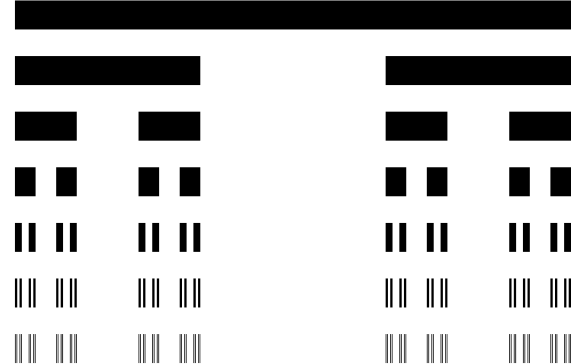
\includegraphics[width=2in]{cantor}$\quad$
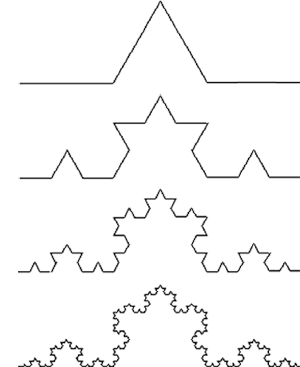
\includegraphics[width=2in]{koch}
}
\Frame{Box Dimension}{
\defin The \emph{Box Dimension} (or Minkowski-Bouligand dimension) of a set $S\in\R^n$ is the limit (if it exists)
$$\Db(S)=\lim_{\epsilon\to0}\frac{-\log N(\eps)}{\log\epsilon},$$
where $\Ne$ is the number of square boxes of side length $\eps$ required to cover the set. 

For any finite sequence $\eps_0>\cdots>\eps_n$, the best-fit slope through the points $\lrp{-\log\eps_k,\log N(\eps_k)}$ is an approximation to $\Db$.
}
\Frame{How to Compute $\Db$}{
Notice in particular that, for any $r>1$, we can set $\eps_k=r^{-k}$ and get
$$\Db(S)=\lim_{k\to\infty}\frac{-\log N(\eps_k)}{\log \eps_k}
=\lim_{k\to\infty} \frac{\log_r N(r^{-k})}{k}.$$
\begin{itemize}
\item
For the Cantor Set $\mc{C}$, with $r=3$ we get $$\Db(\mc{C})=\log2/\log3.$$ 
\item
For the Koch Curve $\mc{K}$, it's easier to see if we use circles (of diameter $\eps$) for our covering set; then with $r=3$ we get  $$\Db(\mc{K})=\log4/\log3.$$
\end{itemize}}
\Frame{Entropy of a Fractal}{
This limit, $\lim_{k\to\infty} \frac{\log_r N(r^{-k})}{k}$, has the same form as the per-symbol entropy of an information source! Here, a ``message of length $k$'' is just a choice of one of the $N(r^{-k})$ covering boxes of side length $r^{-k}$.

Accordingly, we define the \emph{entropy of a fractal} to be 
$$H(S)=\Db(S) \bits.$$
This is the (limiting) amount of information produced each time we ``zoom in'' by a factor of two.
}
\Frame{Entropy of Cantor, Koch}{
	\begin{itemize}
		\item Cantor:
		 $H(\mc{C})=\frac{\log 2}{\log 3}\bits$ (per zoom), or since this works for any $r$, 
			$$
			H(\mc{C})
			\ =\ \frac{\log 2}{\log 3} \ \frac{\text{trits}}{\text{$3x$-zoom}}
			\ =\ 1\  \frac{\text{bit}}{\text{$3x$-zoom}}.
			$$
		Indeed, to zoom in on the Cantor Set by a factor of 3, we must choose ``left'' or ``right'' --- 1 bit of entropy!
		\item Koch:
		Similarly,
		$$
		H(\mc{K})
		\ =\ \frac{\log 4}{\log 3}\bits 
		\ =\   2\ \frac{\text{bits}}{\text{$3x$-zoom}}.
		$$
	\end{itemize}
}


\section{Fractal Image Analysis}
\subsection{The Method}
\Frame{A Photograph}{
Consider a black \& white photograph. There a couple of natural ways to represent this mathematically:
\begin{itemize}
\item As a function, $I:R\subset\R^2\to\R$.
\item For a digital photo, as an $m\times n$ matrix $J$.
\end{itemize}
To analyse it as a fractal, we need a set of points in $\R^2$. In fact, each \emph{threshold value} $t$ induces such a set: define 
$$I_t^{-1}=\lrc{(x,y):|I(x,y)|\leq t},$$
or in the matrix case,
$$J_t^{-1}=\lrc{\lrp{\frac{i}{m},\frac{j}{n}}:|J_{ij}|\leq t}.$$
}
\Frame{Fractal Spectrum}{
\defin
The \emph{fractal spectrum} of an photograph $I$ over a set of threshold values, $S\subset\R$,  is the function $\FS:S\to\R$ given by
$$\FS= \Db(I_t^{-1}).$$
For an image matrix we take an approximation to $\Db$. 

Finally, if $S=\{t_1,\ldots,t_m\}$ is finite, we may write
$$\FS=\lrp{\Db(I_{t_1}^{-1}),\ldots,\Db(I_{t_m}^{-1})}\in\R^m,$$
where typically $t_1<\cdots<t_m$.
}
\Frame{Example}{
\al{\!\!\text{Let }J=\begin{bmatrix}
	4&2&1&3\\
	1&6&1&7\\
	3&2&8&7\\
	4&5&5&6
	\end{bmatrix}.	
	\text{ So with $t=4,$ }
	J_t^{-1}=\begin{bmatrix}
	1&1&1&1\\
	1&0&1&0\\
	1&1&0&0\\
	1&0&0&0
	\end{bmatrix}.}
To compute $\Db(J_4^{-1})$, write $N(1)=1,$ $N(\frac{1}{2})=3,$ and $N(\frac{1}{4})=8.$ The log-log slope comes to approximately $1.585$.

\rule{0em}{2em}Similarly, $\Db(J_2^{-1})\approx1.161$ and $\Db(J_6^{-1})\approx1.850$
}
\Frame{Fractal Excess}{
A high fractal dimension does not necessarily mean an interesting photograph!

In the matrix case, we can compare this photograph to others of the same size and pixel intensity distribution.

\defin
Let $J$ be an image matrix and let $\mc{J}$ be the set of all copies of $J$ with permuted entries. Then the \emph{fractal excess} of $J$ over a threshold set $S$ is the function
$$\FE=\frac{1}{|\mc{J}|}\lrp{\sum_{J'\in\mc{J}}\FS_{J'}}-\FS_J.$$
Again, for finite $S$, we may write $\FE$ as a vector in $\R^m$.
}
\Frame{Examples}{
With $J$ as in the previous example, it turns out that $\FE_J\approx(-10^{-13},10^{-13},-10^{-14})$ over $S=\{2,4,6\}$.

This is small because there's not much room for anything interesting to happen in a 16 pixel photograph.\begin{wrapfigure}{r}{0.5\textwidth}\centering
    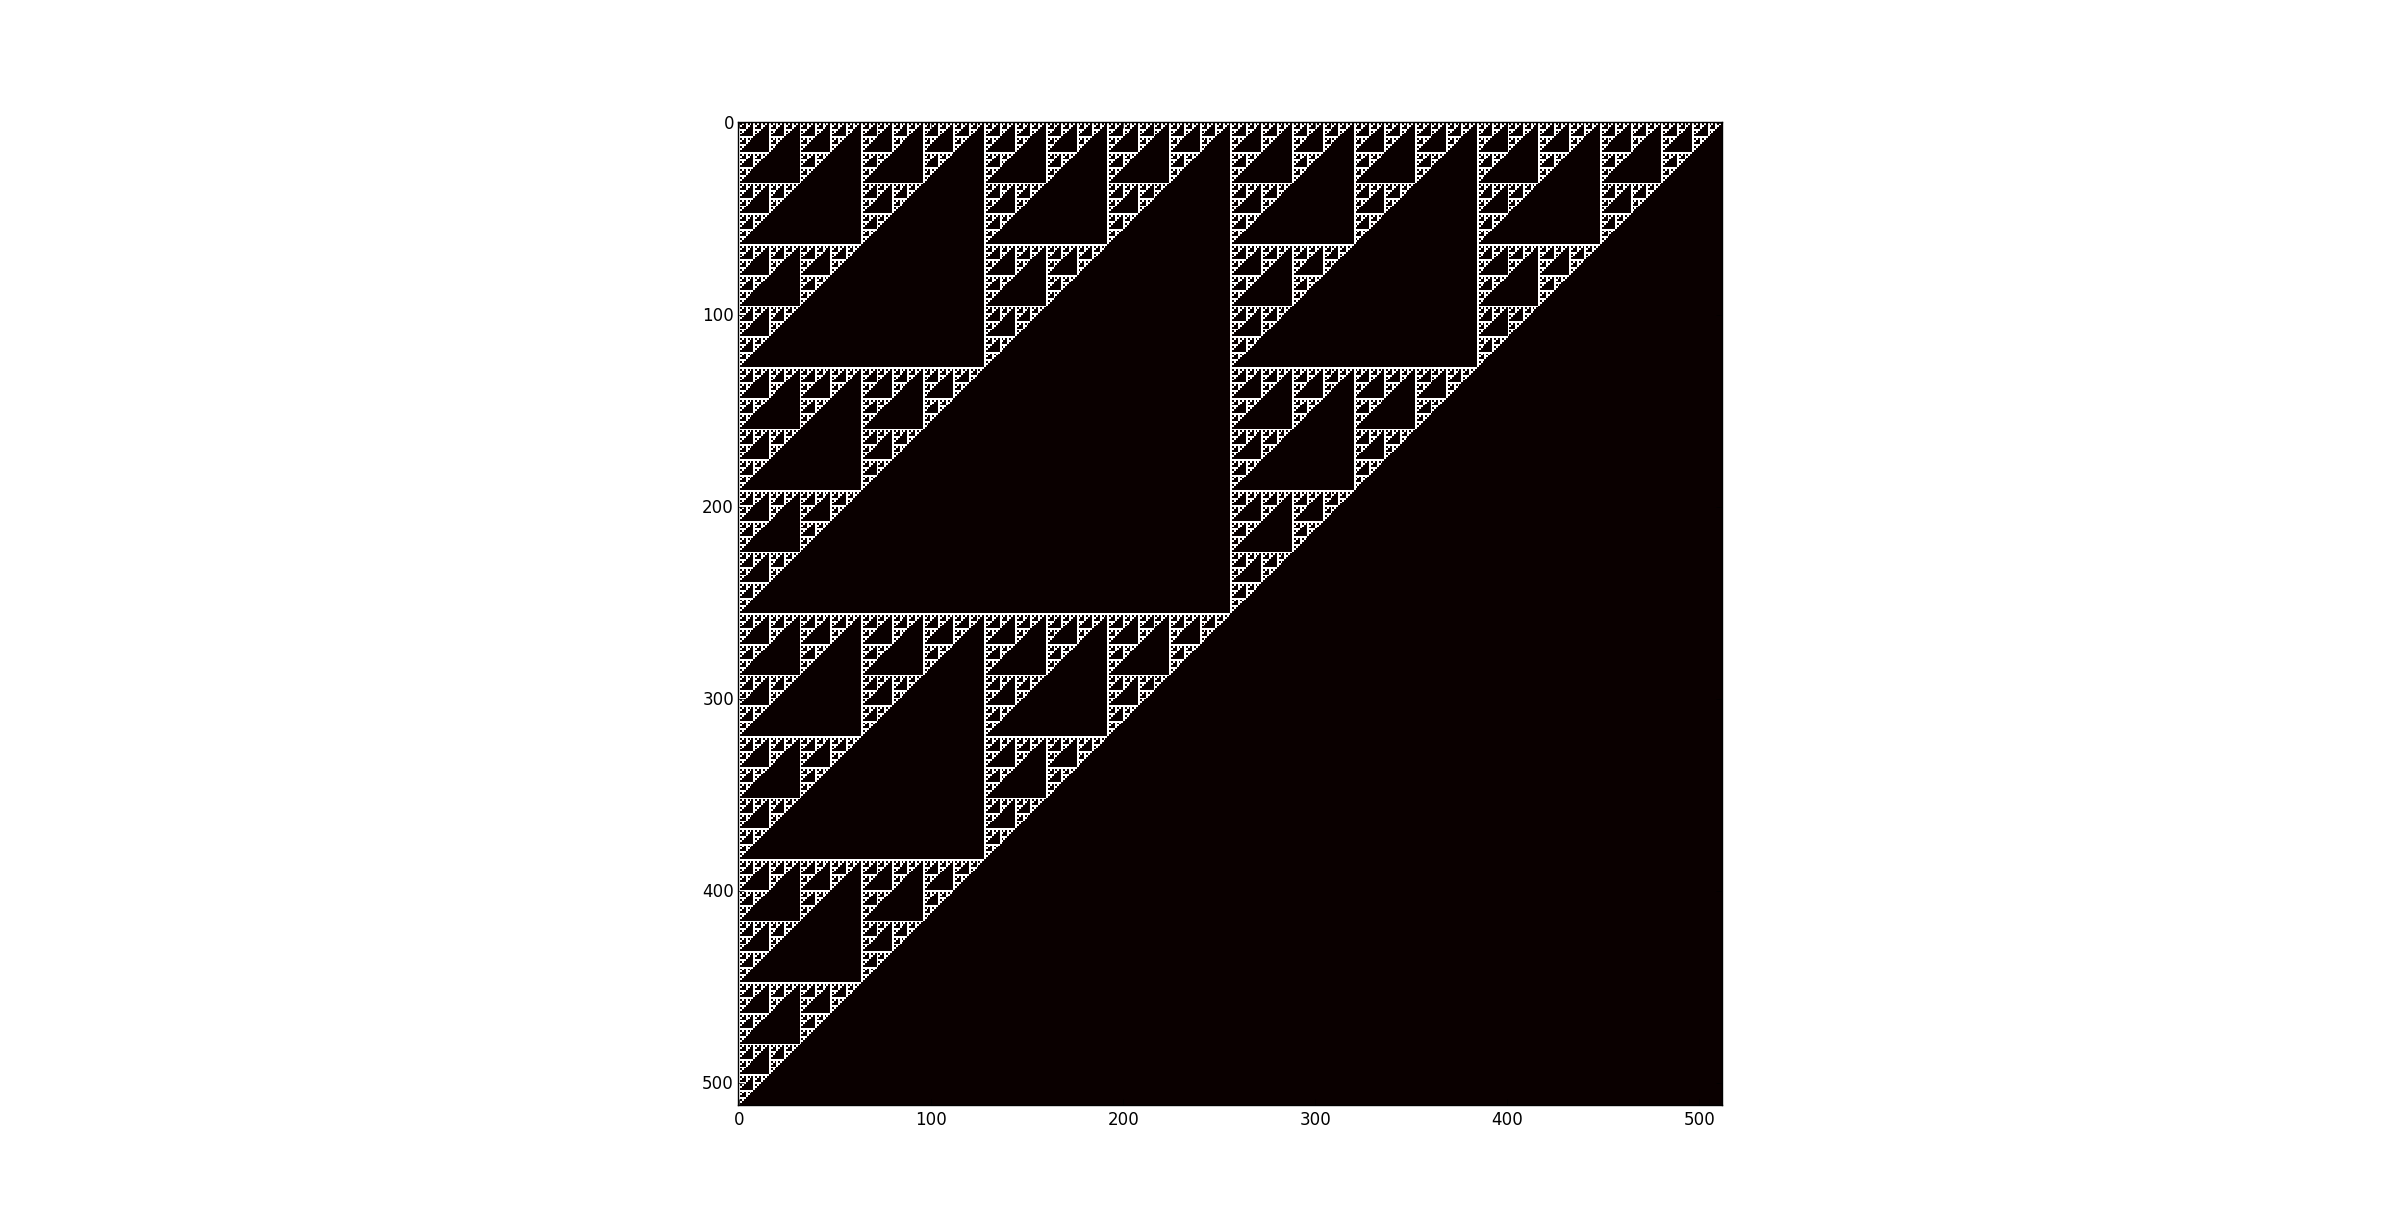
\includegraphics[width=3in]{figure_1}
\end{wrapfigure}

\addtolength{\rightskip}{-6em}
In the {photograph at right}, the dimension\\ is again about $1.585$, but computing the\\ fractal excess using the definition would be\\ impractical; instead the image was compared\\ to a single random permutation of itself.\\ The $\FE$ is about 0.1.
}
\Frame{N.B.}{As that last example shows, the numeric values obtained for $\FE$ are highly dependent on the resolution of your image.}


\subsection{Use in Astrobiology}
\Frame{}{
I return now to the paper\dots
}
\Frame{}{
So it looks like they've shown ($p<0.05$) precisely the opposite of what they set out to show: life exhibits \emph{higher} entropy than visually similar abiotic phenomena!

\rule{0em}{2em}But this really is due to a confusion of definitions. The fractal entropy the authors measure is not the same as the thermodynamical entropy they discuss in their introduction.
}
\Frame{}{
What the authors have shown is some connection between the two; an investigation into that connection would be a logical next step.

\rule{0em}{2em}Intuitively, it seems they're measuring complexity in some nebulously defined sense: a poorly-shuffled (low entropy) deck of cards still has higher entropy than a fair coin toss, simply because there's more going on.
}

\section*{Conclusion}

\begin{frame}{What Next?}
	This project was a blast, and raised a lot of new questions that I'd like to pursue at some point.

  % Keep the summary *very short*.
  \begin{itemize}
  \item
    How good are these approximations to $\Db$ for image matrices?
  \item
	How does this new quantity ``fractal excess'' behave? It clearly depends on the image resolution, but in what way, and can we ``normalize'' for that somehow? Can we compute the average fractal dimension of a scrambled image combinatorially?
  \item
	My reading has hinted at a deep connection between all the various animals called ``entropy'': information theoretic, classical thermodynamic, and statistical thermodynamic. I'm very curious to learn more.
  \item What is the connection between the fractal complexity of a physical object and its physical entropy?
  \end{itemize}
  
\end{frame}
\Frame{Thanks, Edoh!}{
To conclude, I'd like to thank my advisor Edoh Amiran for his invaluable help and support throughout this project.
}


% \section{Introduction}

% %\subsection[Short First Subsection Name]{First Subsection Name}

% \begin{frame}{Make Titles Informative. Use Uppercase Letters.}{Subtitles are optional.}
  % % - A title should summarize the slide in an understandable fashion
  % %   for anyone how does not follow everything on the slide itself.

  % \begin{itemize}
  % \item
    % Use \texttt{itemize} a lot.
  % \item
    % Use very short sentences or short phrases.
  % \end{itemize}
% \end{frame}









% \begin{frame}{Make Titles Informative.}

  % You can create overlays\dots
  % \begin{itemize}
  % \item using the \texttt{pause} command:
    % \begin{itemize}
    % \item
      % First item.
      % \pause
    % \item    
      % Second item.
    % \end{itemize}
  % \item
    % using overlay specifications:
    % \begin{itemize}
    % \item<3->
      % First item.
    % \item<4->
      % Second item.
    % \end{itemize}
  % \item
    % using the general \texttt{uncover} command:
    % \begin{itemize}
      % \uncover<5->{\item
        % First item.}
      % \uncover<6->{\item
        % Second item.}
    % \end{itemize}
  % \end{itemize}
% \end{frame}


\end{document}


